\documentclass[10pt]{exam}
\usepackage[phy]{template-for-exam}
\usepackage{my-tikz-clipart}


\title{Energy \#5}
\author{Rohrbach}
\date{\today}

\begin{document}
\maketitle

\begin{questions}

\question
  A car's speed is cut by 1/3.  By what factor does the car's kinetic energy change?
  \vs

\question
  A car's speed is cut by 1/5.  By what factor does the car's kinetic energy change?
  \vs

\question
  A car has twice the speed of a truck.  However, the truck has four times as much mass.  Which vehicle has a larger kinetic energy?

  \begin{tikzpicture}
    \path (-4,0) coordinate (one) pic[scale=0.5] {car}
      +(1.25, 0.25) node {$m$};
    \draw[->,blue,very thick] 
      (one) ++(2.5,0.25) -- ++(2,0) 
      node[anchor=west] {$2v$};
    \path (4,0) coordinate (two) pic[scale=0.5] {truck}
      +(1.25, .35) node {$4m$};
    \draw[->,blue,very thick] 
      (two) ++(2.5,0.25) -- ++(1,0)
      node[anchor=west] {$v$};
  \end{tikzpicture}
  \vs[2]

\question
  A marble starts at rest at the top of a frictionless ramp with 60 J of potential energy.  How much kinetic energy does it have when it has fallen 2/3 of the way down the ramp?

  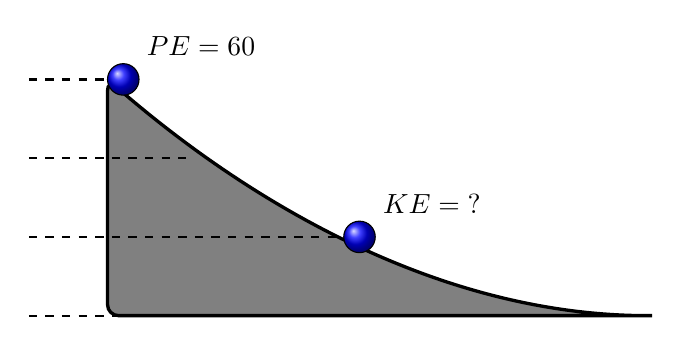
\begin{tikzpicture}
    \draw[very thick, rounded corners,fill=gray] 
      (0,0) -- (0,3) 
      parabola[bend at end] (7,0)
      -- cycle;
    \draw[dashed,thick] (-1,0) -- ++ (8,0);
    \draw[dashed,thick] (-1,1) -- ++ (4,0);
    \draw[dashed,thick] (-1,2) -- ++ (2,0);
    \draw[dashed,thick] (-1,3) -- ++ (1,0);
    \draw[shading=ball] (0.2,3) circle (.2)
      node[above right=5pt] {$PE=\SI{60}{\joule}$};
    \draw[shading=ball] (3.2,1) circle (.2)
      node[above right=5pt] {$KE=\text{ ?}$};
  \end{tikzpicture}
  \vs[2]

\pagebreak

\question
  A loaded mining car has a mass of 1230 kg and is being lifted out of a mine shaft by a winch (a motor attached to a chain).  It takes 240 seconds to lift the mining carthrough a vertical distance of 200 meters.

  \begin{parts}
    \part
      Calculate the work done by the winch.
      \vs 
    
    \part
      Calculate the power output of the winch.
      \vs 

  \end{parts}
  

\question
  A 15-kg cart is moving at 10 m/s at the bottom of a ramp.  How far up the ramp does it get if there is 120~J of work done by friction?
  \vs[2]






\end{questions}

\end{document}